% !TEX TS-program = xelatex
% !TEX options = -shell-escape -synctex=1 -interaction=nonstopmode -file-line-error "%DOC%"
\documentclass{beamer}
\usetheme{metropolis}

% Packages for code formatting
\usepackage{listings}
\usepackage{xcolor}
\usepackage{hyperref}
\usepackage{graphicx}

% Define colors to match the Metropolis theme
\definecolor{metropolis-bg}{RGB}{48,48,48} % Background color
\definecolor{metropolis-text}{RGB}{220,220,220} % Text color
\definecolor{metropolis-keyword}{RGB}{204,204,255} % Keyword color
\definecolor{metropolis-comment}{RGB}{150,150,150} % Comment color
\definecolor{metropolis-string}{RGB}{255,175,150} % String color

% Configure listings to use these colors
\lstset{
    language=Python,
    backgroundcolor=\color{metropolis-bg},
    % basicstyle=\ttfamily\small\color{metropolis-text},
    basicstyle=\tiny\ttfamily\color{metropolis-text}, % Use \tiny for smaller font size
    % basicstyle=\fontsize{5pt}{6pt}\selectfont\ttfamily\color{metropolis-text}, % Custom smaller font size
    keywordstyle=\color{metropolis-keyword}\bfseries,
    commentstyle=\color{metropolis-comment},
    stringstyle=\color{metropolis-string},
    % numbers=left,
    % numberstyle=\fontsize{4pt}{5pt}\color{gray},
    stepnumber=1,
    numbersep=8pt,
    frame=single,
    showstringspaces=false,
    breaklines=true,
    xleftmargin=20pt,
    xrightmargin=20pt,
    columns=fullflexible,
    keepspaces=true,
}

\title{Professional Project Highlights}
\date{\today}
\author{Newell Jensen}
\begin{document}
    \maketitle

    \begin{frame}
        In this presentation, I will provide a brief overview of several projects I've worked on that showcase my experience:
        \begin{itemize}
            \item Canonical Ltd. -- MaaS Redfish Power Driver
            \item ESP32-C3 Nixie Tube Clock
        \end{itemize}
    \end{frame}

    \section{MaaS -- Redfish Power Driver}
    \begin{frame}{Introduction}
        What is MaaS?

        \begin{itemize}
            \item MaaS, or Metal as a Service, is a software framework developed by Canonical, the company behind Ubuntu, that allows you to manage physical servers just like virtual machines in a cloud environment. It automates the provisioning and management of physical servers, enabling them to be treated as a flexible and scalable resource pool.
            \item See: \href{https://maas.io/}{https://maas.io/}
        \end{itemize}


    \end{frame}

    \begin{frame}{Power Drivers}
        Power drivers in MaaS are responsible for managing the power state of the physical servers. They allow MaaS to remotely power on, power off, or reboot servers. This functionality is crucial for automating the deployment and management of physical servers. Different types of power drivers correspond to different methods or protocols used to control the power state of the hardware.
    \end{frame}

    \begin{frame}{Power Drivers}
        Some examples are:
        \begin{itemize}
            \item IPMI (Intelligent Platform Management Interface): A widely used standard for managing server hardware, allowing remote power control, monitoring, and diagnostics.
            \item Redfish: A newer standard for hardware management that uses RESTful APIs, supporting power control and other management functions.
            \item AMT (Intel Active Management Technology): A hardware and firmware technology that allows remote management of computers, including power control.
            \item Wake-on-LAN (WoL): A protocol that allows a computer to be powered on or awakened from a low-power state by a network message.
        \end{itemize}
    \end{frame}


    \begin{frame}{Redfish Power Driver -- Asynchronous I/O}
        MaaS uses Twisted, an event-driven network programming framework used for asynchronous I/O.
        \scriptsize
        \begin{itemize}
            \item \textbf{Decision}: The code leverages the Twisted framework for handling asynchronous I/O operations, particularly HTTP requests to the Redfish endpoints.
            \item \textbf{Reasoning}: Twisted's event-driven architecture is well-suited for scenarios where multiple I/O-bound tasks need to be performed concurrently, such as sending and receiving HTTP requests without blocking. This is crucial in a system like MAAS, where managing power states across potentially hundreds of nodes needs to be efficient and non-blocking.
            \item \textbf{Alternatives}: Blocking I/O operations or using threads for concurrency. These alternatives could lead to inefficient resource usage or complexity in managing multiple threads, particularly in a high-scale environment.
            \item \textbf{Why Better}: Asynchronous I/O with Twisted allows the system to scale better by managing resources efficiently and reducing the overhead associated with thread management.
        \end{itemize}
    \end{frame}

    \begin{frame}[containsverbatim]
        \frametitle{Twisted Intro -- Making an Asynchronous HTTP Request}
        Before looking at the code of the Redfish Power Driver, let's quickly go over how to make HTTP requests asynchronously using Twisted.

        Twisted provides the \textbf{\texttt{Agent}} class to make HTTP requests. Here's a simple example of how to use it:

        \begin{lstlisting}
            from twisted.internet import reactor
            from twisted.web.client import Agent
            from twisted.web.http_headers import Headers
        \end{lstlisting}
    \end{frame}

    \begin{frame}[containsverbatim]
        \frametitle{Twisted Intro -- Making an Asynchronous HTTP Request}
        Continued...
        \begin{lstlisting}
            def handle_response(response):
                print("Response code:", response.code)
                return response

            def handle_error(failure):
                print("Request failed:", failure)
                reactor.stop()

            def stop_reactor(_):
                reactor.stop()

            agent = Agent(reactor)
            d = agent.request(
                b'GET',
                b'http://httpbin.org/get',
                Headers({'User-Agent': ['Twisted']}), None)

            d.addCallback(handle_response)
            d.addErrback(handle_error)
            d.addBoth(stop_reactor)

            reactor.run()
        \end{lstlisting}
    \end{frame}

    \begin{frame}[containsverbatim]
        \frametitle{Twisted Intro -- Making an Asynchronous HTTP Request}

        \noindent In this example:
        \begin{itemize}
            \item \textbf{\texttt{Agent}} is used to make an HTTP GET request.
            \item The \textbf{\texttt{request}} method returns a \textbf{\texttt{Deferred} (\texttt{d})} that represents the result of the HTTP request.
            \item \textbf{\texttt{addCallback(handle\_response)}} registers the \texttt{handle\_response} function to be called when the request completes successfully.
            \item \textbf{\texttt{addErrback(handle\_error)}} registers the \texttt{handle\_error} function to be called if the request fails.
            \item \textbf{\texttt{addBoth(stop\_reactor)}} ensures that the reactor is stopped after the request is handled, regardless of success or failure.
            \item The \textbf{\texttt{reactor.run()}} call starts the Twisted event loop.
        \end{itemize}
    \end{frame}

    \begin{frame}[containsverbatim]
        \frametitle{Twisted Intro -- Handling HTTP Responses}

        You can read the body of the response asynchronously as follows:

        \begin{lstlisting}
            from twisted.web.client import readBody

            def handle_response(response):
                print("Response code:", response.code)
                d = readBody(response)
                d.addCallback(print_body)
                return d

            def print_body(body):
                print("Response body:", body)
            \end{lstlisting}
            \begin{itemize}
                \item \textbf{\texttt{readBody(response)}} is used to asynchronously read the response body.
                \item \textbf{\texttt{print\_body}} is a callback that prints the response body.
                \item The \textbf{\texttt{handle\_response}} function returns a new \textbf{\texttt{Deferred}} that represents the body read operation, allowing the reactor to wait for it to complete before stopping.
            \end{itemize}
    \end{frame}

    \begin{frame}[containsverbatim]
        \frametitle{Twisted Intro -- Error Handling}

        Twisted uses \textbf{\texttt{Errbacks}} for error handling. If an error occurs in any part of the Deferred chain, it is passed to the registered errback function.
        \begin{lstlisting}
            def handle_error(failure):
                print("Request failed:", failure)
                if failure.check(ConnectionRefusedError):
                    print("Connection refused")
                reactor.stop()
            \end{lstlisting}
            \noindent The \textbf{\texttt{handle\_error}} function:
            \begin{itemize}
                \item Prints the error.
                \item Uses \textbf{\texttt{failure.check()}} to determine the type of error. For example, if the connection is refused, it prints a specific message.
                \item Stops the reactor, which is necessary to end the program.
            \end{itemize}
    \end{frame}

    \begin{frame}[containsverbatim]
        \frametitle{Twisted Intro -- inlineCallbacks}
        Twisted's \textbf{\texttt{inlineCallbacks}} decorator allows you to write asynchronous code in a synchronous style, making it easier to follow. Here's how to rewrite the previous example:

        \begin{lstlisting}
            from twisted.internet.defer import inlineCallbacks

            @inlineCallbacks
            def make_request():
                try:
                    response = yield agent.request(
                        b'GET',
                        b'http://httpbin.org/get',
                        Headers({'User-Agent': ['Twisted']}), None)
                    print("Response code:", response.code)
                    body = yield readBody(response)
                    print("Response body:", body)
                except Exception as e:
                    print("Request failed:", e)
                finally:
                    reactor.stop()

            reactor.callWhenRunning(make_request)
            reactor.run()
            \end{lstlisting}
    \end{frame}

    \begin{frame}
        \frametitle{Twisted Intro -- inlineCallbacks}

        \noindent In this example:
        \begin{itemize}
            \item \textbf{\texttt{inlineCallbacks}} allows the use of \textbf{\texttt{yield}} to wait for Deferreds. This makes the code look more like standard synchronous Python.
            \item \textbf{\texttt{try/except/finally}} handles success and failure, making the error handling clearer.
            \item \textbf{\texttt{reactor.callWhenRunning(make\_request)}} schedules the request to be made when the reactor starts.
        \end{itemize}
    \end{frame}

    \begin{frame}
        \frametitle{Twisted Intro -- Summary}
        This introduction to Twisted has demonstrated the basics of using Twisted for asynchronous HTTP requests, including handling responses and errors. The key points include:
        \begin{itemize}
            \item Using \textbf{\texttt{Deferreds}} to manage asynchronous results.
            \item Adding callbacks and errbacks to handle success and failure.
            \item Using \textbf{\texttt{inlineCallbacks}} to write asynchronous code in a more readable, synchronous style.
        \end{itemize}

        With these tools, you can build efficient, non-blocking network applications using Twisted.
    \end{frame}

    \begin{frame}
        \frametitle{Redfish Power Driver -- Code}

        Now, let's take a quick look at the code for the Redfish Power Driver.

        The code is too long to paste in these slides so let's jump over to my screen and take a look in the GitHub repository...

        NOTE: \href{https://github.com/canonical/maas/blob/master/src/provisioningserver/drivers/power/redfish.py}{\underline{Click to code here}}.
    \end{frame}

    \section{ESP32-C3 Nixie Tube Clock}

    \begin{frame}
        \frametitle{ESP32-C3 Nixie Tube Clock -- Clock}

        \centering
        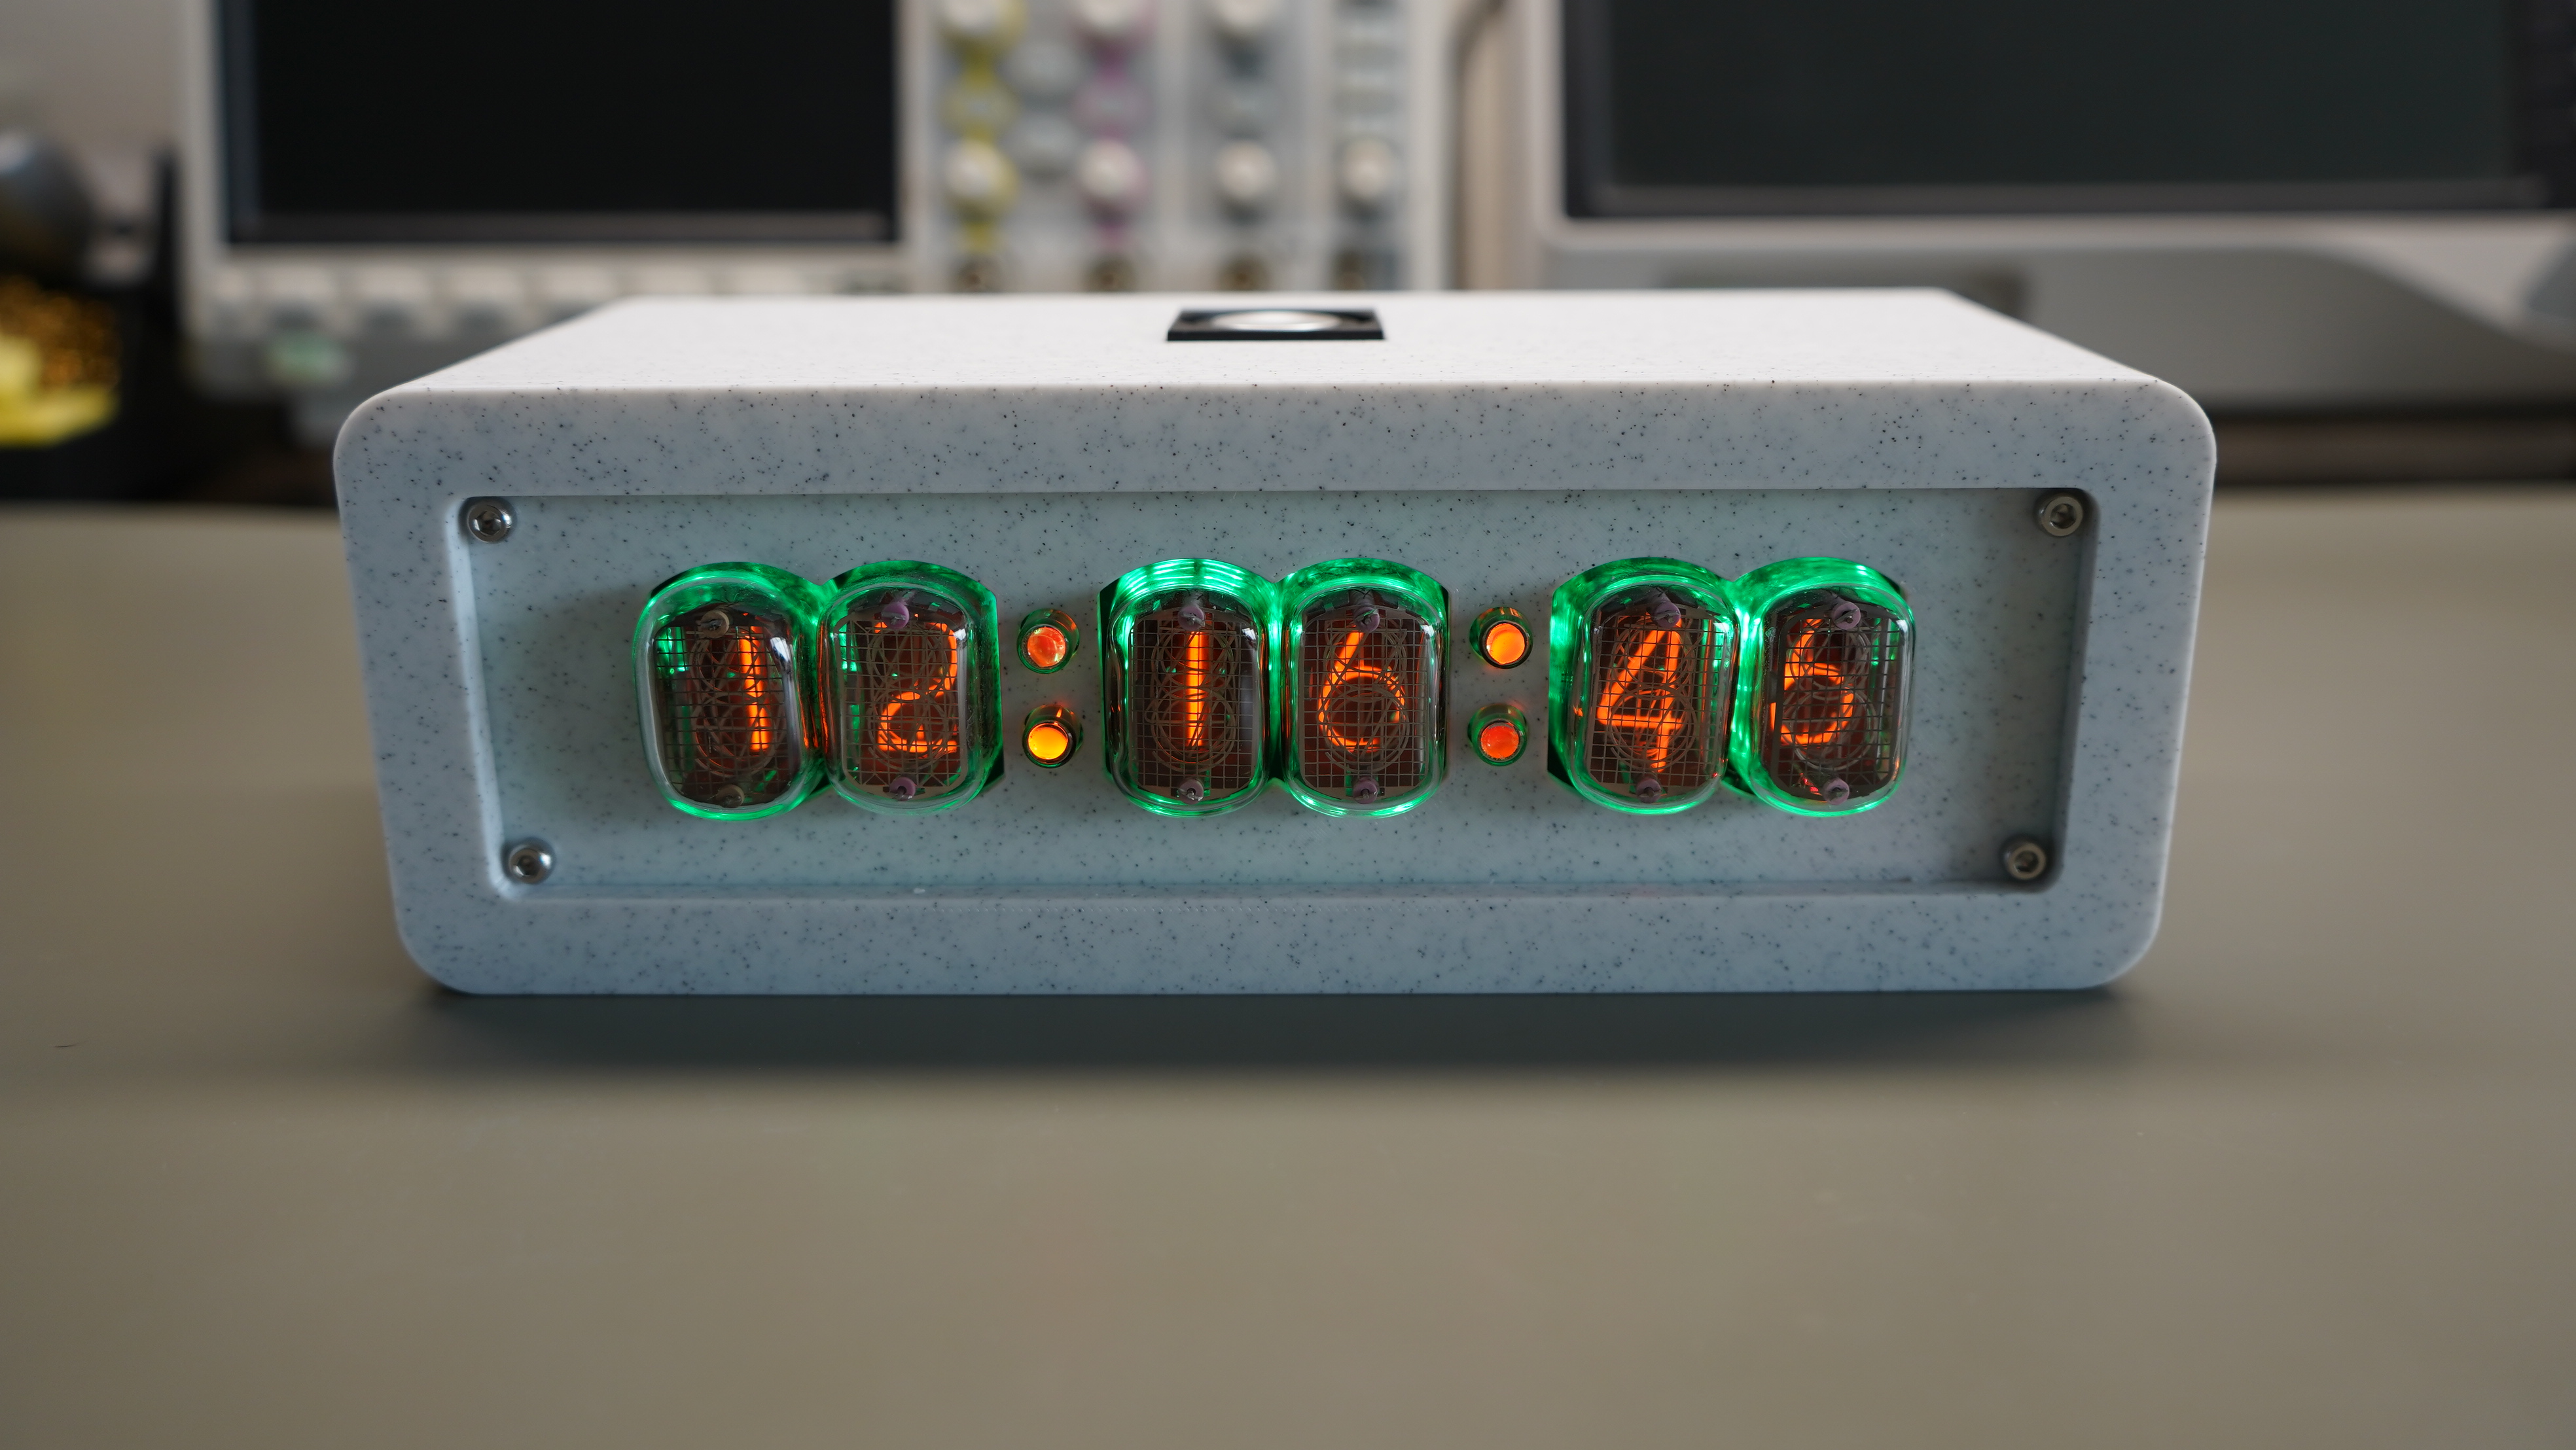
\includegraphics[width=0.8\textwidth]{clock.jpeg}
    \end{frame}

    \begin{frame}{ESP32-C3 Nixie Tube Clock -- Features}
        \footnotesize
        \begin{itemize}
            \item CAD 3D Model of Case and Components using build123d
            \item Six IN-12A Nixie Tubes and Four Colon Indicators
            \item ESP32-C3 microcontroller
            \item Powered via USB-C
            \item High Voltage Flyback Converter
            \item WiFi Provisioning via Bluetooth
            \item Sound
            \item Motion Sensing for Sleep Mode
            \item Webserver and Client to Control Settings:
            \begin{itemize}
                \item WiFi Credentials
                \item 12-hour or 24-hour format
                \item NTP server
                \item Colon Indicators (Blinking, Always On, Off)
                \item Color of LEDs
                \item Timezone
            \end{itemize}
        \end{itemize}
    \end{frame}

    \begin{frame}
        \frametitle{ESP32-C3 Nixie Tube Clock -- Let's Take a Closer Look}

        Let's jump over to my screen so that we can take a closer look at the project!

        NOTE: \href{https://github.com/newell/nixie-clock-esp32c3}{\underline{Click to the repository here}}.

    \end{frame}

\end{document}
